\documentclass{crypto-exercise}
\usepackage{amsthm}
\usepackage{pgfplots}
\usepackage{tikz}

\author{Sven Laur}
\contributor{Kristiina Rahkema}
\editor[Small changes in the presentation]{Sven Laur}
\tags{conditional probabilities, independence, conditional independence}

\newcommand{\HEAD}{\mathsf{head}}
\newcommand{\TL}{\mathsf{tail\text{-}light}}

\begin{document}
\begin{exercise}{Independence of biased coin throws}
Consider an experiment where we first choose a biased coin from the box and then throw the selected coin four times. The box contains two types of coins: tail light and tail heavy coins.  The probability of heads is $90\%$ for a tail light coins and $10\%$ for tail heavy coins. The probability of choosing a tail light coin is unknown. Compute the conditional probability $\pr{\HEAD_2|\HEAD_1}$ and and explain whether two throws of the coin are independent or not. Are two throws of the coin independent if we know whether the coin is tail light or tail heavy? Compute the probability that all four coins are heads. Estimate the probability of the same event form below if we do not know anything about the coins. Instead, we we know that if we choose a coin and throw it then the probability of obtaining head is $50\%$.
\end{exercise}
\begin{solution}
Let $p$ denote the probability that we get a tail-light coin out of the box. Then the probability that the first coin lands on heads is
\begin{align*}
\pr{\HEAD_1} &= p\cdot0.9 + (1-p)\cdot 0.1 = 0.8p+0.1\enspace.
\end{align*}
At the same time, the probability of obtaining two heads in the row is
\begin{align*}
\pr{\HEAD_1\wedge \HEAD_2} &= p\cdot 0.9\cdot 0.9 + (1-p)\cdot 0.1\cdot 0.1  = 0.8p + 0.01\enspace. 
\end{align*}
Therefore, we can express the conditional probability as follows:
\begin{equation*}
\pr{\HEAD_2|\HEAD_1}=\frac{\pr{\HEAD_1\wedge \HEAD_2}}{\pr{\HEAD_1}}%
=\frac{0.8p+0.01}{0.8p+0.1} = 1- \frac{0.09}{0.8p+0.1}\enspace.
\end{equation*}
By using the total probability formula and event decomposition, we can estimate 
\begin{align*}
\pr{\HEAD_2} &= p\cdot 0.9\cdot 0.9 + p\cdot 0.1\cdot 0.9 + (1-p)\cdot 0.1 \cdot 0.1 + (1-p)\cdot 0.9\cdot 0.1 
= 0.8p + 0.1\enspace.
\end{align*}
It is easy to see that the first and the second coin toss are not independent, as the equation $\pr{\HEAD_2}=\pr{\HEAD_2|\HEAD_1}$ does not hold in general. To study this phenomenon more deeply, let us study the ratio
\begin{align*}
\gamma=\frac{\pr{\HEAD_2|\HEAD_1}}{\pr{\HEAD_2}}=\frac{0.8p+0.01}{(0.8p+0.1)^2}=1+\frac{0.64p(1-p)}{(0.8p+0.1)^2}\enspace.
\end{align*}
From the form it is clear that $\gamma>1$, which means that probability of obtaining two heads is always larger than the probability of two heads if the throws would be independent, see Figure~\ref{fig:overrepresentation}. Since initial conditions are symmetrical for heads and tails, the same reasoning shows that the probability of obtaining two tails is also overrepresented compared to the independent model. As a result, probabilities of obtaining different outcomes must be smaller than under independence assumption. The latter is an expected result, as the selected coin is strongly biased we should get the preferred value with higher probability.    


\begin{figure}[!h]
\begin{center}
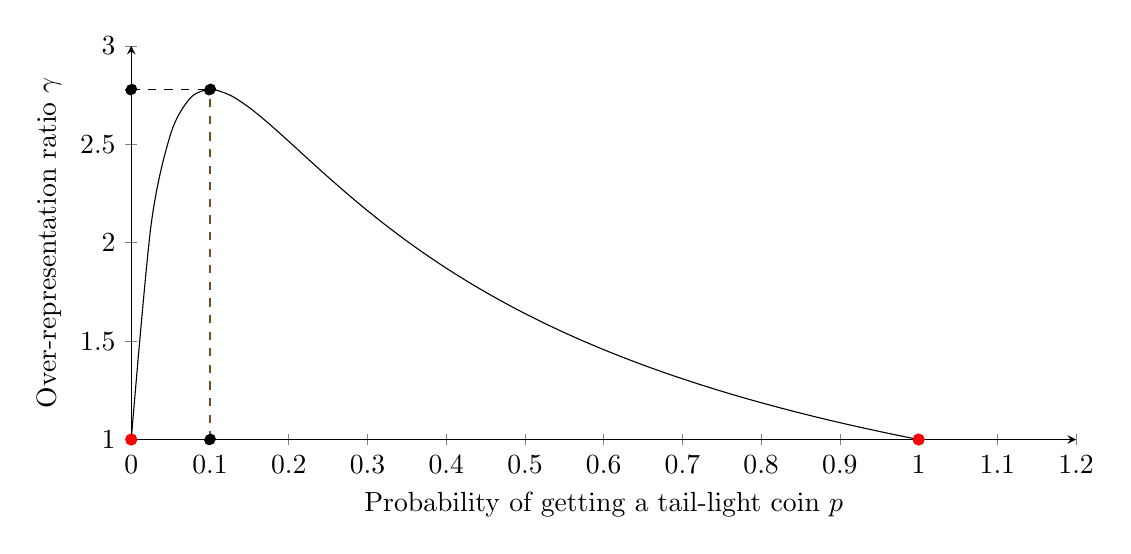
\begin{tikzpicture}
\begin{axis}[
%	scale=1.00,
    y = 2.5cm,
	x = 10cm,
    axis x line =bottom,  % only show the bottom x axis line, without an arrow tip
    axis y line =left,
    xmin=0, xmax=1.2,  % range for the x axis
    ymin=1, ymax=3, 
    xlabel = {Probability of getting a tail-light coin $p$},
    ylabel = {Over-representation ratio $\gamma$},
]

\addplot [smooth]
table
{
0.000000 1.000000
0.025000 2.083333
0.050000 2.551020
0.075000 2.734375
0.100000 2.777778
0.125000 2.750000
0.150000 2.685950
0.175000 2.604167
0.200000 2.514793
0.225000 2.423469
0.250000 2.333333
0.275000 2.246094
0.300000 2.162630
0.325000 2.083333
0.350000 2.008310
0.375000 1.937500
0.400000 1.870748
0.425000 1.807851
0.450000 1.748582
0.475000 1.692708
0.500000 1.640000
0.525000 1.590237
0.550000 1.543210
0.575000 1.498724
0.600000 1.456599
0.625000 1.416667
0.650000 1.378772
0.675000 1.342773
0.700000 1.308540
0.725000 1.275952
0.750000 1.244898
0.775000 1.215278
0.800000 1.186998
0.825000 1.159972
0.850000 1.134122
0.875000 1.109375
0.900000 1.085663
0.925000 1.062925
0.950000 1.041103
0.975000 1.020145
1.000000 1.000000
};

\addplot  [mark=*, mark options = black, style = dashed] 
	coordinates {(0.000000, 2.777778) (0.100000, 2.777778)}
;
\addplot+ [mark=*, mark options = black, style = dashed] 
	coordinates {(0.100000, 1.000000) (0.100000, 2.777778)}
;
\addplot+ [mark=*, mark options = red] 
	coordinates {(1.000000, 1.000000) (0.000000, 1.000000) }
;
\end{axis}
\end{tikzpicture} 
\end{center}
\caption{Over-representation ratio $\gamma$ as a function of selection probability $p$. The ratio decreases when the choice of tail light coin becomes more certain and becomes one if the choice is certain.}
\label{fig:overrepresentation}
\end{figure}


Now let us assume that we know which coin was chosen.  Without loss of generality we can assume that we chose a tail-light coin. Then by definition 
\begin{align*}
\pr{\HEAD_1|\TL}= \pr{\HEAD_2|\TL} =0.9
\end{align*}
and by description of the experiment
\begin{align*}
\pr{\HEAD_1\wedge\HEAD_2|\TL}= \pr{\HEAD_1|\TL} \pr{\HEAD_2|\TL} =0.81\enspace.
\end{align*}
Hence, the coin-tosses are indeed independent if we know the type of the coin. Note that for $p=1$ we know that the tail-light coin is always chosen and thus the over-representation coefficient $\gamma(1)=1$. The same reasoning also gives that $\gamma(0)=1$. These conditions are indeed met, see Figure~\ref{fig:overrepresentation}. 


The probability that in four throws all coins land on the head is 
\begin{align*}
\pr{\HEAD_1\wedge\ldots\wedge\HEAD_4} &= p\cdot 0.9^4 + (1-p)\cdot 0.1^4\enspace. 
\end{align*}
For example, $\pr{\HEAD_1\wedge\ldots\wedge\HEAD_4}=0.3281$ if both coin types are equiprobable: $p=0.5$.

\vskip 3ex
\noindent\textsc{Box with unknown coins.}
In this setting we do not know what kind of coins are in the box. We just know that if we take a random coin then the probability of getting a head as an outcome is $50\%$. Let us assume that there are $n$ different types of coins $x_1,\ldots,x_n$ that occur with probabilities $p_1,\ldots,p_n$. Also assume that the coin $x_i$ lands on head with probability $\lambda_i$. Then
\begin{align*}
\pr{\HEAD_1}=\sum_{i=1}^n{p_i\lambda_i}=0.5
\end{align*}
by assumption. Now we can express the probability of for heads as follows:
\begin{align*}
\pr{\HEAD_1\wedge\ldots\wedge\HEAD_4} &= \sum_{i=1}^n \pr{x_i\wedge \HEAD_1\wedge\ldots\wedge\HEAD_4} 
= \sum_{i=1}^n p_i \lambda_i^4\enspace.
\end{align*}
Note that this holds, as the trows become independent if we know the type of coin. As $x^4$ is a convex-cup function, Jensen's inequality assures that
\begin{align*}
\pr{\HEAD_1\wedge\ldots\wedge\HEAD_4} &=\sum_{i=1}^n p_i\lambda_i^4\geq \left( \sum_{i=1}^n{p_i\cdot \lambda_i}\right)^4 
= 0.5^4 = 0.0625\enspace.
\end{align*}
This means that the probability throwing four heads in a row is at least $0.0625$ given that the probability of throwing one head is $0.5$. The bound is quite loose in general. Above, we established that if tail-heavy and tail-light coins are equiprobable then $\pr{\HEAD_1}=0.5$ and $\pr{\HEAD_1\wedge\ldots\wedge\HEAD_4}=0.3281$, which is much larger than our lower bound $0.0625$.  
\end{solution}
\end{document}

